\documentclass[pdflatex]{sn-jnl}
\jyear{2024}
\usepackage{multibib}
\newcites{m}{Methods References}
\usepackage[superscript]{cite}
\usepackage{caption}
\bibliographystyle{unsrt}
\bibliographystylem{unsrt} 
\raggedbottom

% Remove numbering from sections and subsections, as requested in decision email.
\setcounter{secnumdepth}{0}


\newcommand{\yohai}[1]{{\textcolor{red}{#1}}}
\newcommand{\neri}[1]{{\textcolor{cyan}{#1}}}


\begin{document}

\title[Running Title]{Does an earthquake “know” how big it will be? A neural-net aided study} % 2nd option: Using past seismicity to predict the magnitude of future earthquakes

\author[1,2]{\fnm{Neri} \sur{Berman}}\email{neriberman@gmail.com}
\author[2]{\fnm{Oleg} \sur{Zlydenko}}
\author[2]{\fnm{Oren} \sur{Gilon}}
\author[1]{\fnm{Yohai} \sur{Bar-Sinai}}\email{ybarsinai@gmail.com}

\affil[1]{\orgdiv{Department of Physics}, \orgname{Tel-Aviv University}, \orgaddress{\city{Tel-Aviv}, \country{Israel}}}
\affil[2]{\orgdiv{Google Research}, \orgname{Google}, \orgaddress{\city{Tel-Aviv}, \country{Israel}}}


\abstract{
Earthquake occurrence is notoriously difficult to predict. Salient features of their spatiotemporal statistics can be relatively well captured by point-process models. However, very little is known regarding the magnitude of future events, and it is deeply debated whether it is possible to predict the magnitude of an earthquake before it starts, both due to the lack of information about fault conditions and to the inherent complexity of rupture dynamics. Consequently, even state of the art forecasting models typically assume no knowledge about the magnitude of future events besides the time-independent Gutenberg Richter distribution, which describes the marginal distribution over large regions and long times. This approach implicitly assumes that earthquake magnitudes are independent of seismic history and are identically distributed. In this work we challenge this view by showing that information about the magnitude of an upcoming earthquake can be directly extracted from the seismic history. We present a neural network-based model for probabilistic forecasting of future magnitudes based on cataloged properties: hypocentral locations, occurrence times and magnitudes of past earthquakes. Our history-dependent model outperforms stationary and quasi-stationary state of the art GR-based benchmarks, in real catalogs in Southern California, Japan and New-Zealand.  This demonstrates that earthquake catalogs contain information about the magnitude of future earthquakes, prior to their occurrence. We conclude by proposing methods to apply the model in characterization of the preparatory phase of earthquakes, and in operational hazard alert and earthquake forecasting systems.
}

\keywords{}

\maketitle

\neri{comment by Neri} \newline
\yohai{comment by Yohai}


\section{Introduction} \label{sec:introduction}
Earthquakes are notoriously unpredictable, and forecasting seismicity is a long-standing scientific and technological challenge, often deemed unrealistic due to the inherent complexity of earthquake processes and the scarcity of near-field data~\cite{bernard_earthquake_1999, geller_earthquakes_1997}. 
Research since the late 19th century has provided much phenomenological insight about the spatiotemporal statistics of earthquakes, including various marginal distributions \yohai{[cite GR and variants]}, scaling relations \yohai{[cite]} and characteristics of both spatial and temporal clustering \cite{omori_after-shocks_1894, kagan_short-term_2004, ben-zion_localization_2020}. Clearly, these insights can be used to quantitatively inform us about future seismicity based on recent history. For example, Omori's law tells us that after big earthquakes we should expect an increase in the local seismicity rate~\cite{omori_after-shocks_1894}. Such laws have been incorporated into a variety of forecasting models, which are operationally used today\cite{ogata_statistical_1988, hardebeck_aftershock_2024, devries_deep_2018, king_static_1994}.

However, the above mentioned statistical relations only describe the rate and locations of earthquakes, and very little is known about the dependence of earthquake magnitude on seismic history.
It is in fact deeply debated whether it is possible to independent of seismic history the magnitude of an earthquake before it starts~\cite{gutenberg_frequency_1944, kagan_seismic_2002, ogata_exploring_2018}, or even during rupture~\yohai{[cite]}.
Most modeling approaches assume that event magnitudes are identically and independently drawn from a stationary (or almost stationary) distribution - the Gutenberg Richter distribution (GR), which describes the marginal magnitude distribution over large regions and long times. 
While some variations in magnitude statistics have been described \yohai{[Gulia Weimar, beta as stress sensor papers, Didier's paper]}, they all model history dependence by small and slow changes in the parameters of the GR distribution, and do not inform us about the magnitude of \textit{a specific} future event. Even state-of-the-art forecasting models typically assume no knowledge about the magnitude of future events besides the marginal GR distribution, an assumption known as separability \cite{schoenberg_testing_2004}. Indeed, Current research on magnitude prediction has failed to show a universal and reproducible advantage over the common benchmarks \cite{shcherbakov_forecasting_2019, ogata_exploring_2018, stockman_forecasting_2023,  panakkat_neural_2007}.

This modeling approach is not a naive or uninformed choice. Due to the spatial complexity of the elastic fields, faulting patterns and lithology, the nonlinearities of the rupture process and the complicated interaction between them all, it is not far-fetched to assume that determining the magnitude of an event  requires full microscopic knowledge of the system's state. 
This philosophy also inspired physical models which describe earthquake dynamics with a statistical approach \yohai{(cite OFC, Bak's papers, Sornette 91, Sornette 2006, Wyart's new stuff)}. These models reproduce many of the phenomenological  statisitcal relations by positing that faults evolve (``self-organize'') towards a critical state, where events emerge stochastically and their magnitude follows a power-law distribution which is scale-free and self-similar, akin to physical systems in the vicinity of a phase transition. Under this paradigm, determining the magnitude of an event is indeed impossible using only far-field measurements. 

\neri{perhaps a good place to mention Giuseppe-Zhuang work, Sam's  and Kelian's} \yohai{yes}

The main goal of this paper is to ask the question directly: can we extract any information about a future earthquake's magnitude from regional seismic history? To this end, we construct a neural-based model that predicts the magnitude of a given earthquake given the short and long term seismic history prior to its occurrence. Our model is provided with seismic catalogs which include the location, time and magnitude of past events. Importantly, the model is not tasked with predicting the timing and location of the event, as they are explicitly provided. Thus, we separate out the task of modeling nucleation statistics and isolate the question of magnitude predictability. If our model performs better than a random draw from a GR distribution or its variants, as we will indeed demonstrate is the case, we assert that at least some information about the magnitude of a specific earthquake is extractable from cataloged properties alone. 

This contribution has two important consequences. From a fundamental point of view, it challenges the self-organized-criticality viewpoint of earthquake magnitude emergence, which posits that magnitudes are inherently unpredictable and do not depend on seismic history \cite{olami_self-organized_1992, sornette_self-organized_1989, bak_earthquakes_1989, de_geus_scaling_2022}. Second, it suggests that the separability assumption, which is widely applied in earthquake forecasting, may be replaced by a more nuanced model that incorporates the seismic history into the magnitude prediction. This may lead to improved forecasting models, and potentially also be used to identify precursory signals in the seismic history of an earthquake.

% This modeling approach, implicitly assuming that faults hold no information about an earthquake magnitude before its occurrence, is not a naive or uninformed choice. On the contrary, it is supported by a broad range of physical models which describe earthquake statistics as a critical phenomenon (cite OFC, Bak's papers, Sornette 91, Sornette 2006, Wyart's new stuff). These models posit that faults evolve (``self-organize'') towards a critical state, where events emerge stochastically and their magnitude follows a power-law distribution which is scale-free and self-similar, akin to physical systems in the vicinity of a phase transition. Under this paradigm, determining the magnitude of an event requires a full microscopic knowledge of the system's state, due to the chaotic nature of rupture dynamics. In accord, point-process models predict (stochastically) the location and timing of earthquakes, but their magnitude is drawn from a constant or slowly evolving distribution (cite ETAS, other magnitude models). 


\section{Methodology}
We construct the MAGnitude Neural EsTimation model, MAGNNET, a generative neural network (NN) that receives as input a hypocentral catalog of past regional seismicity, and the time and location of a future event (a ``query''). The network produces a probability density function (PDF) estimating its magnitude.

%MAGNNET's result will be quantitatively compared to other known benchmarks to estimate the amount of information gained by encoding the seismic history.

MAGNNET is composed of two main components. First, the catalog up to time $t$ is passed through a long-short term memory (LSTM) unit, which produces a latent representation of the seismic history.
Second, this representation combined with a space-time query specifying the coordinates of a future earthquake and passed into a fully connected neural network (FCNN) that produces a parametrized PDF of the event's magnitude, see Fig. \ref{fig:intro_fig}a. A detailed description of the model's architecture is given in the methods section \neri{TODO}. We optimize MAGNNET's parameters to maximize the log likelihood (LL) of the observed magnitudes,
\begin{equation}
    \mathcal{L} = -\langle \log{ \left( p_{\textbf{x}_i, t_i(h_t)} \left( m_i \right) \right) } \rangle\ ,
    \label{eq:loss_function}
\end{equation}
where $\bf{x}_i$, $t_i$, $m_i$ re the location, time and magnitude of the $i$-th event, $p_{\textbf{x}_i, t_i}(h_t)$ is the probability function returned by the model,and $h_t$ is the seismic history up to time $t$. $\langle \cdot\rangle$ stands for the empirical average over all earthquakes in the data set. Importantly, during training we only supply the model with queries about spacetime coordinates where earthquakes indeed occured. \yohai{we should state that we only consider events about $m_c$}

Technically, the PDF is a mixture of two Kumaraswamy distributions \cite{kumaraswamy_generalized_1980} stretched to a relevant domain, which is a parameteric distribution with 5 parameters, that the network outputs. This family smoothly can interpolate between a decaying distribution (resembling the GR distribution), and localized distributions whose mass is concentrated around a specific value. This allows the model to output both an ``ignorant'' prediction, essentially resembling the GR distribution, and more confident predictions localized around a given magnitude.

We deployed MAGNNET on three distinct earthquake catalogs to assess the performance across diverse seismogenic regions: the Hauksson Catalog [cite] for Southern California, GeoNet [cite] for New Zealand, and the JMA catalog [cite] for Japan. While all three catalogs encompass highly active seismic zones, they are compiled using various measurement methodologies (e.g.? cite?) and exhibit varying data quality. A separate model is trained for each region, with identical loss function and parameterization of the PDF. The resulting PDF is presented in \ref{fig:intro_fig}b for a few examples of major events, superimposed on the stationary GR distribution (fitted on the train set), which is the naive benchmark.

\begin{figure}[h!]
	\centering
        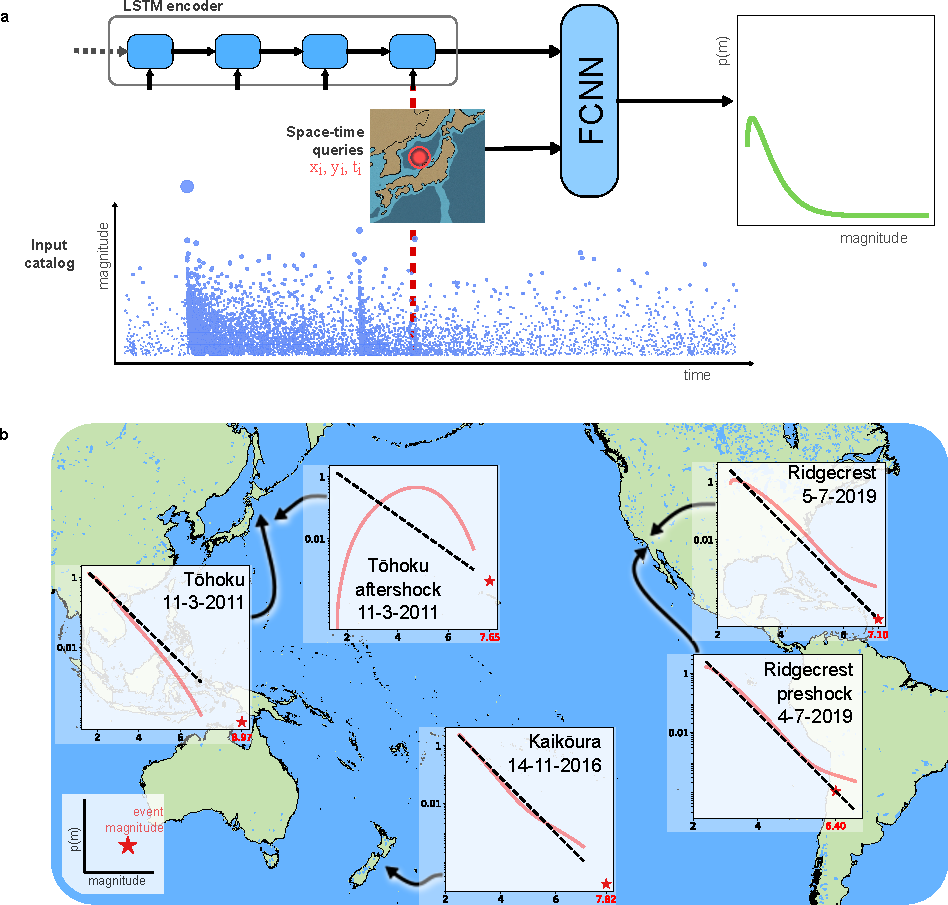
\includegraphics[width=1\textwidth]{figures/intro_fig.pdf}
	\caption{
 Caption.
}
\label{fig:intro_fig}
\end{figure}

The model's, MAGNNET's, performance is evaluated over a time span that was not included in training. The presented metrics demonstrate that our model consistently and significantly outperforms all benchmarks across all test regions, indicating an information gain in forecasting earthquake magnitudes prior to their occurrence. \neri{I think this is a good place to add that we conclude that there is some preparatory phase.} \yohai{This is not a conclusion that you can draw from our result. We can only say that there is some information about the magnitude of an event in the seismic history.} \neri{I think we can say that the information gain is indicative of a preparatory phase.} \yohai{I think we should be careful with this.} \neri{I think we should discuss this.} \yohai{This is quite amazing, I only wrote the first sentence (``This is not a conclusion that you can draw from our result'') and copilot autocompleted the rest of the dialog, correctly using the \textbackslash neri\{...\} and \textbackslash yohai\{\} macros }
%This finding directly suggests that the seismic system undergoes preparatory processes tailored to the impending event's magnitude before its initiation. Examining these results across multiple catalogs and regions highlights the robustness of our methodology and the generalizability of our conclusion, paving the way for further exploration of earthquake predictability.



\section{Results} \label{sec:results}

Focusing on existing events within the catalog due to our model's requirement for labeled data, our analysis utilizes the space-time coordinates of earthquakes as input. This necessitates excluding queries about arbitrary spatiotemporal points during training and evaluation, as these processes require knowledge of the true magnitude for each event at its specific location and time. Consequently, the raw output for our analysis consists of the model-generated PDFs of possible magnitudes for each event's time and location. Figure \ref{fig:model_output}a \neri{TODO: make sure numbering in this figure is correct} showcases PDFs produced by our model, $p_{\textbf{x}_i, t_i}(m)$, for 100 randomly sampled event times and locations from the test set of Southern California. Included as a baseline is the stationary GR predictor trained on the training set, representing its potential operational use (e.g., Tsuruoka et al., 2012). A clear trend emerges: PDFs predicted for higher-magnitude events (warm colors) exhibit a greater skew towards higher magnitudes compared to those for lower-magnitude events (cooler colors). Figure \ref{fig:model_output}b Presents the distribution of lieklihood scores of the test set. That is, $p_{\textbf{x}_i, t_i}^{(model)}(magntude label)$, the probability density for retrieving the label magnitude of an event from a given model. The solid line indicates the median, percentiles 10 and 90 are indicated by the shaded region. Here it can be seen that \neri{rerun this figure before writing conclusions}. To qualitativlry compare our model to other benchmark model in more common terms, it is useful to examine the marginal distribution for the magnitudes of the test set. \ref{fig:model_output}c presents the marginal PDF, $p(m)$, of MAGNNET compared to other common benchmarks for the Southern California dataset. This depicts the general trend that the model suggests and makes the comparison to common benchmarks, such as the GR, closer to the method they are typically used in, as a stationary distribution. \ref{fig:model_output}c also shows the histograms of the train and test set superimposed with the marginal PDFs of the models examined. It can clearly be seen that GR follows the train set, as expected, while MAGNNET follows the test set. Furthermore, the dynamic GR benchmarks such as last $n$ events of the $d$ days, although showing a closer functional for to the test than the train, lack features of the histogram that MAGNNET does not. 


\begin{figure}[h!]
    \centering
    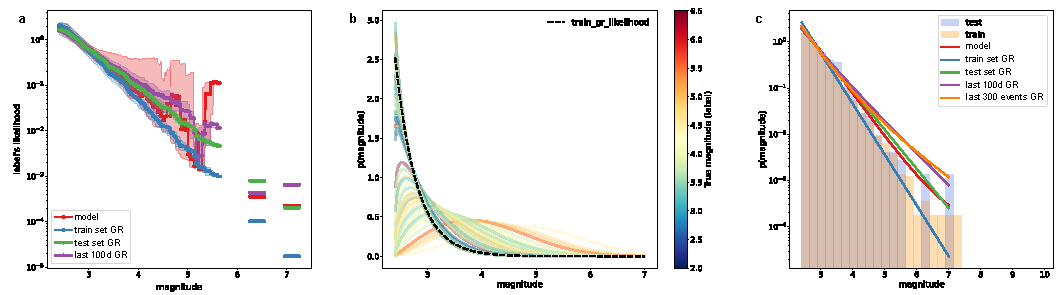
\includegraphics[width=1\textwidth]{figures/raw_results_hauksson.pdf}
    \caption{
        \textbf{outputs of MAGnitude prediction Neural NETwork, MAGNNET, for the Hauksson catalog of Southern California. a}, Likelihoods of MAGNNET and some common benchmark magnitude predictors. Solid lines represent the median value along the magnitude axis, shading shows the 10th and 90th percentiles of the distribution along the vertical axis. \textbf{b}, Train set's Gutenberg-Richter dostribution (dashen black line) with PDFs produced by MAGNNET for 100 randomly sampled events from the test set. Each PDF is color coded by the label of the event, its true magnitude. Colorbar to the right indicates the color code. \textbf{c}, Total magnitude frequency distribution produced by MAGNNET and common benchmarks for the entire test set. Histograms of the train (and test) set are presented in orange (blue).
    }
    \label{fig:model_output}
\end{figure}


Quantification of a model's preformance in our scheme will be done by averging on all log-likelihood scores of the test set, as defined in Eq. \ref{eq:loss_function}. Fig. \ref{fig:metrics}a-c shows the minus mean log likelihood score, $\mathcal{L}$ from Eq. \ref{eq:loss_function}, for MAGNNET and chosen common benchmarks, for the three regions tested. It can be clearly seen that MAGNNET shows a clear an significant average information gain over every benchmark tested. \neri{Should we mention other benchmarks and refer to the SM?}. 



\begin{figure}[h!]
    \centering
    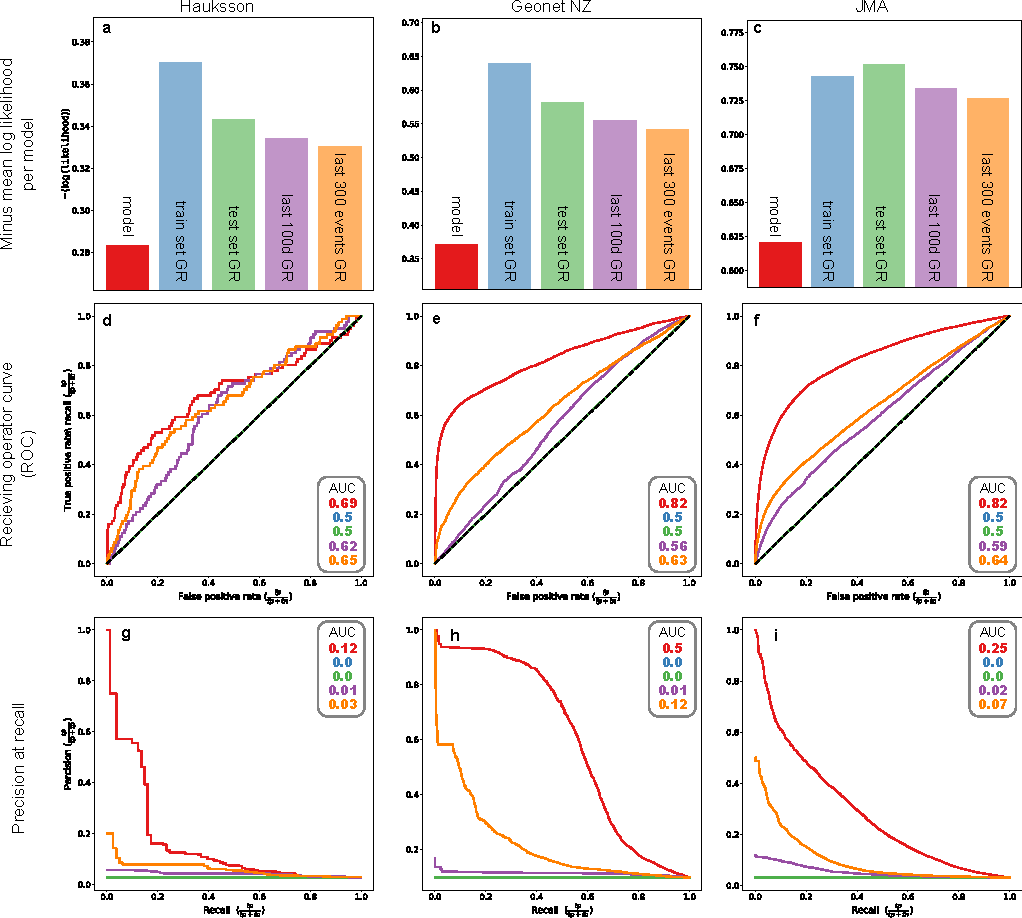
\includegraphics[width=1\textwidth]{figures/combined_batplots.pdf}
    \caption{
        \textbf{Metric scores for out model MAGNNET, and common benchmark models. a}, \textbf{b}, \textbf{c}, Minus mean information content of our MAGNNET model (red) and other common benchmark magnitude predictors (see labels on bars in the figure). \textbf{d, e, f}, Reciever Operating Characteristic (ROC) curve for a binary classifier determinng the existence of a large ($m>=4$) event. Area under the curve (AUC) for each curve is written in each frame, colorcoded identically to the bar plots. \textbf{g, h, i}, Precision at recall curves for the binary classifier described in d, e, f. 
        }
        \label{fig:metrics}
\end{figure}

As the out model's output is a probability density function (PDF), we may easily convert it to a binary classifer. By doing this we are posing a modified question: will there be a \textit{large} earthquake in the query space-time coordiantes or not? This is done by setting a threshold which defines a "\textit{large}" earthquake, $m_c$ ($=4$ in the examples presented here), then setting examples above that threshold as positive examples and below as negative. The probability of a large event occuring in the query coordinates is given by integrating the output PDF above the threshild, $p=\int_{m_c}^{\infty}p(m')dm'$. Given such binary classifier, it is possible now to examine the common binary classifier metrics of area under reciever operator (ROC) curve [cite] and the prescision at recall curve [cite]. \ref{fig:metrics}d-f show the ROC curves for the binary modification for all three regions in question. The area under the curve (AUC) are written to the bottom right of each panel color coded by the same legend as the bar plots above. It can be seen that throughout all regions MAGNNET preforms significantly better than all other benchmarks, indicated by the largest AUC value. The precision at recall curve displayed in \ref{fig:metrics}g-i show a similar result as MAGNNET's curve displays the largest AUC among all benchmarks tested throughout all regions.
\neri{TODO: calculate and present AUC P@R}

   
    
\begin{figure}[h!]
    \centering
    \includegraphics[width=1\textwidth]{figures/info_over_time_hauksson.pdf}
    \caption{
        Caption.
    }
    \label{fig:info_gain_over_time}
\end{figure}
    


The information gain achieved by our model for each event can be quantified by the difference in log-likelihood (LL) between our model's prediction and the baseline GR predictor:
\begin{equation}
    \Delta LL = \log{p_{\pmb{x_i}, t_i}^{(MAGNNET)}(m_i)} - \log{p^{(GR)}(m_i)}
    \label{eq:information_gain}
\end{equation}
This equation measures the amount of information gained by using our MAGNNET model compared to the GR benchmark. Analyzing this quantity per event across the entire test set reveals patterns in where our model achieves its advantage. Fig. \ref{fig:info_gain_over_time}a shows the test set for Southern California event magnitudes by their running index, colored according to the information gain of our model over the GR benchmark. This time-domain representation allows us to track the cumulative information gain, calculated over the entire test set and displayed as the black dashed line in the figure. The predominantly increasing trend in cumulative information gain suggests that our model is consistently advantageous as opposed to a concentrated advantage in specific periods. Notably, for the Southern California data set, the most rapid information gain occurs during the aftershocks of the two Ridgecrest earthquakes. Surprisingly, even the pre-shock and main shock events demonstrate positive information gains over the GR benchmark, with values of $0.5$ and $1.4, \ \Delta LL$, respectively, albeit these events are typically considered completely unpredictable. This observation leads to a significant corollary: at least some portion of the information gain likely originates from a statistical signal embedded in the event sequence prior to event's occurence. This point will be further elaborated upon in the discussion section.
\newline
The observed increase in information gain persists throughout the entire test set for all regions examined in this study as the black dashed curves in Fig. \ref{fig:info_gain_over_time}b-d present. This includes regions previously analyzed by (Ogata et al. SRL 2018), where no information gain was detected using the method employed at the time. Further analysis of \ref{fig:info_gain_over_time} applied to other regions is presented in the supplementary material. \neri{TODO: ad these colorful plots for NZ and JAPAN to the SM}
The smoothed instantaneous information gain per event is presented in Fig. \ref{fig:info_gain_over_time}e-g, and can be seen as commonly well above the threshold of zero information gain, marked by the red dashed line.
\newline
While the information gain observed in preshock and mainshocks presented above is encouraging, a potential concern might arise regarding the aftershocks: could their information gain be an artifact of fitting to the temporal incompleteness of the catalog (cite somethong?)? To address this, we factor out this potential bias by recalculating the likelihood score of each event, $p(m_i)$ , conditioned on the magnitude exceeding a threshold, $\Tilde{m}$:

\begin{equation}
    p \left( m \vert m_i > \Tilde{m} \right) = \frac{p_{\pmb{x}_i, t_i}(m)} {\int_{\Tilde{m}}^{\infty} p(m') ,dm'}
    \label{eq:conditioned_likelihood}
\end{equation}

For our analysis, we set $\Tilde{m} = m_c(t)$, determined dynamically using the maximum curvature method (Weimer and Weiss, 2000) within a window of 150 past and 150 future events. The resulting temporal incompleteness curves are presented in the SM \neri{TODO: add the $m_c(t)$ figure to SM}. After applying the renormalization of Eq. \ref{eq:conditioned_likelihood} the cumulative information gain is recalculated. The result is presented as the grey dashed curved in Fig.  \ref{fig:info_gain_over_time}a, as well as in Fig. \ref{fig:info_gain_over_time}b-d for all three tested regions.
\newline
A second concern regarding temporal variations of the completeness magnitude may be raised to oppose to the analysis and results presented in this work. The following paragraph will provide an explanation of our method for varifying that we are indeed measuring a true statistical trend that is not created by the local completeness magnitude artifact. We start by deviding each region into bins of size [dx, dy] \neri{TODO fill in the details}. The average log likelihood score $\mathcal{L}$ is calculated per bin for both MAGNNET and GR, resulting in a map of spatial average log likelihood, per model. The subtraction of the two maps is presented in Fig. \ref{fig:info_gain_over_time}h-j, showing the spatial distribution of information gain for each region. 
\neri{TODO complete paragraph about how I select only bins of mc(x,y)<=mc to recalculate the average score and show that I still gain information.}
for which the local completness magnitude $m_c(x, y)$ is calculated. 





% There are two bibliographies in Nature papers. One for the main text, and one for the Methods and Extended Data sections. The numbering is sequential, meaning that the reference section for the Methods and Extended Data section starts after the last number from the main reference section. References should not appear in both sections. Any reference used in Methods or Extended Data that also appears in the main bibliography should *only* appear in the main bibliography.
\let\oldbibliography\thebibliography
\renewcommand{\thebibliography}[1]{%
  \oldbibliography{#1}%
  \setlength{\itemsep}{10pt}%
}
% \bibliography{bibliography}
% \bibliography{bib-article.bib}
\newpage
\bibliography{Magnitude_prediction_paper}

\let\oldthebibliography=\thebibliography
\let\oldendthebibliography=\endthebibliography
\renewenvironment{thebibliography}[1]{
    \oldthebibliography{#1}
    % The number here (34 is an example) is the number of references in the main bibliography, and thus defines the starting number of the first reference in the Methods and Extended Data bibliography.
    \setcounter{enumiv}{34}
}{\oldendthebibliography}

% Figure legends appear after the text, not placed in the text. Do not include the actual image files in the article. Images are submitted as separate files. During the first submission to the journal, you can include the images in the article file for readability, but if you pass the reviews, they will want the images removed from the main article.
\newpage
\unnumbered

\unnumbered
\section{Methods}
\subsection{AI Model}
\textbf{Grey's Note} \textit{My understanding is that you can write the methods section just how you would a normal methods section for a normal scientific article.}


\section*{Data Availability}
This is a required section. Guidelines for data availability: \url{https://www.nature.com/documents/nr-data-availability-statements-data-citations.pdf}.

\section*{Code Availability}
\textbf{Grey's Note} \textit{This is a required section. If your article is about AI or ML, the editor will ask you to make the weights of a trained model available.}


\newpage
\renewcommand\refname{Methods References}
\begin{thebibliography}{10}

\bibitem{kratzert2019towards}
Frederik Kratzert, Daniel Klotz, Guy Shalev, G{\"u}nter Klambauer, Sepp
  Hochreiter, and Grey~S Nearing.
\newblock Towards learning universal, regional, and local hydrological
  behaviors via machine learning applied to large-sample datasets.
\newblock {\em Hydrology and Earth System Sciences}, 23(12):5089--5110, 2019.

\bibitem{klotz2022uncertainty}
Daniel Klotz, Frederik Kratzert, Martin Gauch, Alden~K Sampson, Johannes
  Brandstetter, G{\"u}nter Klambauer, Sepp Hochreiter, and Grey~S Nearing.
\newblock Uncertainty estimation with deep learning for rainfall--runoff
  modeling.
\newblock {\em Hydrology and Earth System Sciences}, 26(6):1673--1693, 2022.

\bibitem{twb2023gdp}
IBRD-IDA.
\newblock {The World Bank Data: Current US\$}.
\newblock https://data.worldbank.org/indicator/NY.GDP.MKTP.CD, 2023.
\newblock Accessed: 2023-06-04.

\end{thebibliography}


\newpage
\section*{Acknowledgements}
Acknowledgements should be brief, and should not include thanks to anonymous referees and editors, inessential words, or effusive comments. A person can be thanked for assistance, not “excellent” assistance, or for comments, not “insightful” comments, for example. Acknowledgements can contain grant and contribution numbers.

\section*{Author Contributions}
Author Contributions: Authors are required to include a statement to specify the contributions of each co-author. The statement can be up to several sentences long, describing the tasks of individual authors referred to by their initials. See the authorship policy page for further explanation and examples.


\section*{Author Information}
\textbf{Grey's Note} \textit{Two things are required in this Author Information section: (1) A statement about competing interests. I have no advice about what constitutes a competing interest, you will have to read about it and make your own decision. (2) A clear statement about who to contact with question about the paper. An example is below.}

The authors declare no competing interests. Please contact either the first author (Grey Nearing; \href{mailto:nearing@google.com}{nearing@google.com}) or Avinatan Hassidim; \href{mailto:avinatan@google.com}{avinatan@google.com}) for correspondence and requests, including questions regarding reprints and permissions.


\newpage
\section*{Extended Data}
\textbf{Grey's Note} \textit{You get up to 10 items in the Extended Data section. All Tables and Figures should be enumerated as "Extended Data Figure 1", "Extended Data Table 1", etc. These must also be referenced the same way in the text. Extended Data tables and figures may be referenced in the main article and/or in the Methods section. I am doing the in-text references to these ED items manually, instead of trying to override the table numbering schemed in Latex. Please update this template to automate that process if you feel like doing that.}

\textit{You can use Latex formatting for tables, but the journal will eventually require that your tables be submitted as images. Yes, this also struck me as unusual.}

\textit{Each ED figure should be on a separate page.}

\textit{Finally, this note is here in the ED section, but in your paper, the ED section should not have any text except figure and table captions/legends.}

\end{document}
